\documentclass[11pt]{article}
\usepackage[utf8]{inputenc}
\usepackage[T1]{fontenc}
\usepackage[margin=1in]{geometry}
\usepackage{graphicx}
\usepackage{float}
\usepackage{caption}
\usepackage{subcaption}
\usepackage{booktabs}
\usepackage{hyperref}
\usepackage{placeins}
\usepackage{amsmath}

\title{\textbf{Chile's Peripheral Macroeconomic History:\\Central Bank Solvency, External Leverage, and Structural Balance-of-Payments Vulnerability (1920--2024)}}
\author{Dissertation Pipeline: Chapter 2}
\date{\today}

\begin{document}

\maketitle

\section*{Overview and Analytical Framework}

This monograph compiles the full quantitative visual record of Chile's monetary solvency, external balance-sheet leverage, and structural balance-of-payments vulnerability across the twentieth and twenty-first centuries (1920--2024). It combines high-frequency Central Bank historical balance sheets (from the ClioLab-UC database, 1926--2010) with the comprehensive Nievas \& Piketty (2025) World Historical Balance of Payments (WBOP) database (1920--2024).

The historical analysis is structured around four major institutional and monetary transitions:
\begin{itemize}
    \item \textbf{1931 (Suspension of Convertibility)}: The collapse of the Kemmerer gold-standard orthodoxy following the Great Depression and the collapse of British sterling, forcing the state to introduce administrative foreign-exchange controls.
    \item \textbf{1942 (The Institutional Pivot -- Law 7,200)}: The formal replacement of commercial reserve backing with functional central-bank credit expansion, establishing the state-led Import Substitution Industrialization (ISI) regime under CORFO.
    \item \textbf{1973 (Military Coup \& Neoliberal Shock)}: The violent dismantling of ISI, unilateral tariff liberalization, and the transition to private external debt-led accumulation culminating in the catastrophic 1982 financial crash.
    \item \textbf{1989 (Central Bank Autonomy \& Free-Floating Neoliberalism)}: The institutionalization of autonomous inflation-targeting, capital account liberalization, and the absorption of the 2004--2011 copper super-cycle under financial subordination.
\end{itemize}

\FloatBarrier
\section{Central Bank Solvency and Domestic Leverage (1926--2010)}

\begin{figure}[H]
    \centering
    \caption{\textbf{Solvency Ratios by Monetary Aggregate in Chile (1926--2010)}}
    \label{fig:solv_combined}
    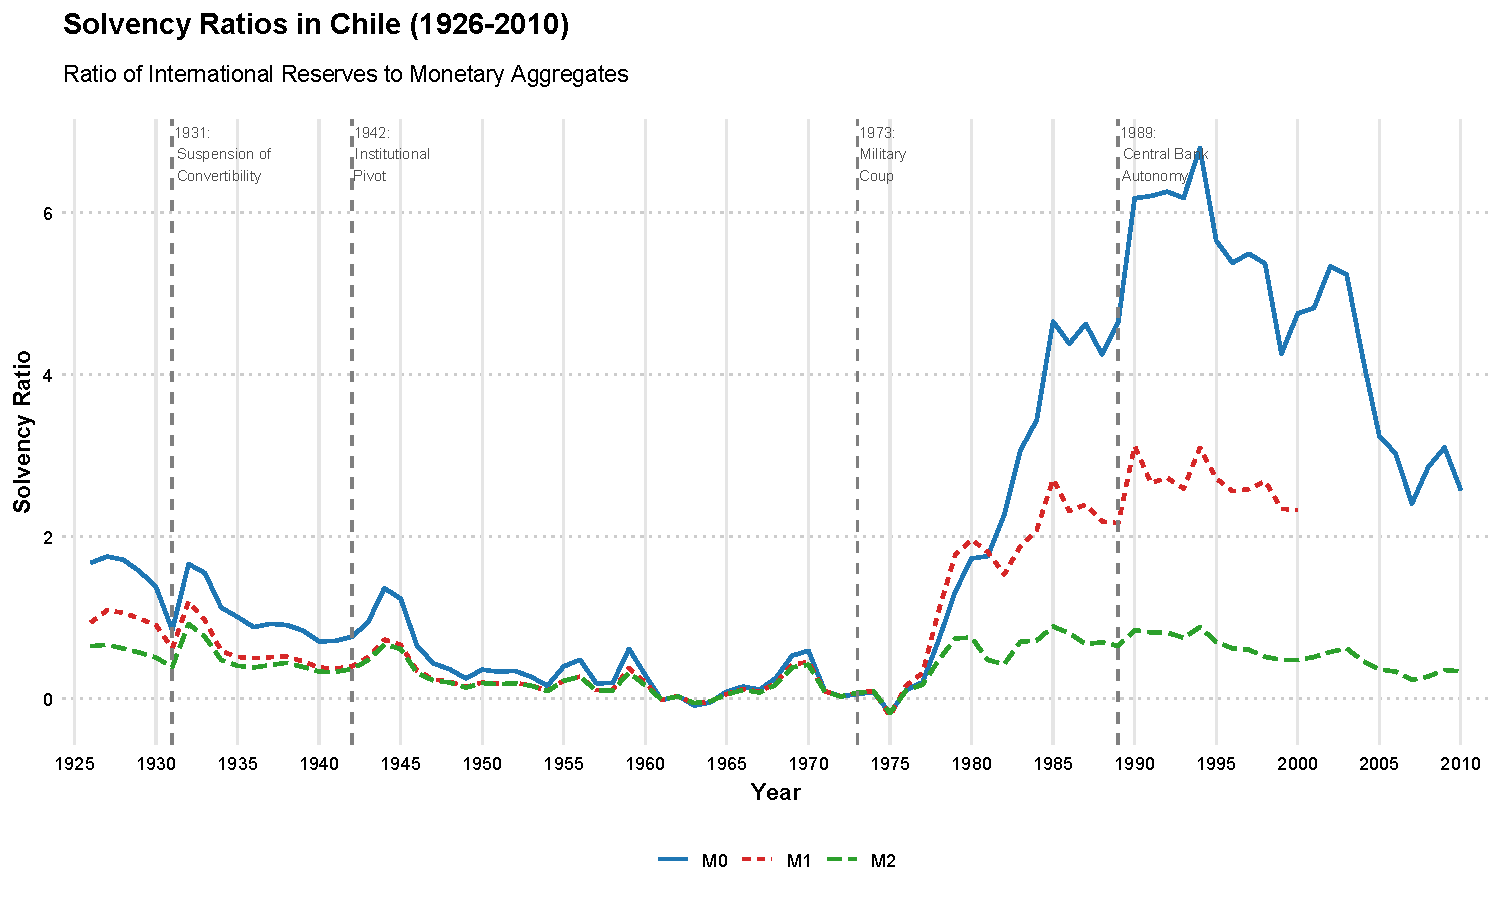
\includegraphics[width=\textwidth]{fig_solv_combined.pdf}
    \vspace{0.3cm}
    \begin{minipage}{\textwidth}
        \footnotesize \textit{Notes:} Solvency ratio defined as International Reserves (converted to nominal Chilean Pesos at the official exchange rate) divided by the corresponding domestic monetary aggregate ($M_0, M_1, M_2$). Colored lines distinguish liquidity tiers: $M_0$ (monetary base), $M_1$ (narrow money), and $M_2$ (broad money). Vertical dashed lines demarcate major institutional regime breaks (1931, 1942, 1973, 1989). Source: ClioLab-UC and Banco Central de Chile.
    \end{minipage}
\end{figure}

\begin{figure}[H]
    \centering
    \caption{\textbf{Domestic Leverage Ratios by Monetary Aggregate in Chile (1926--2010)}}
    \label{fig:lev_combined}
    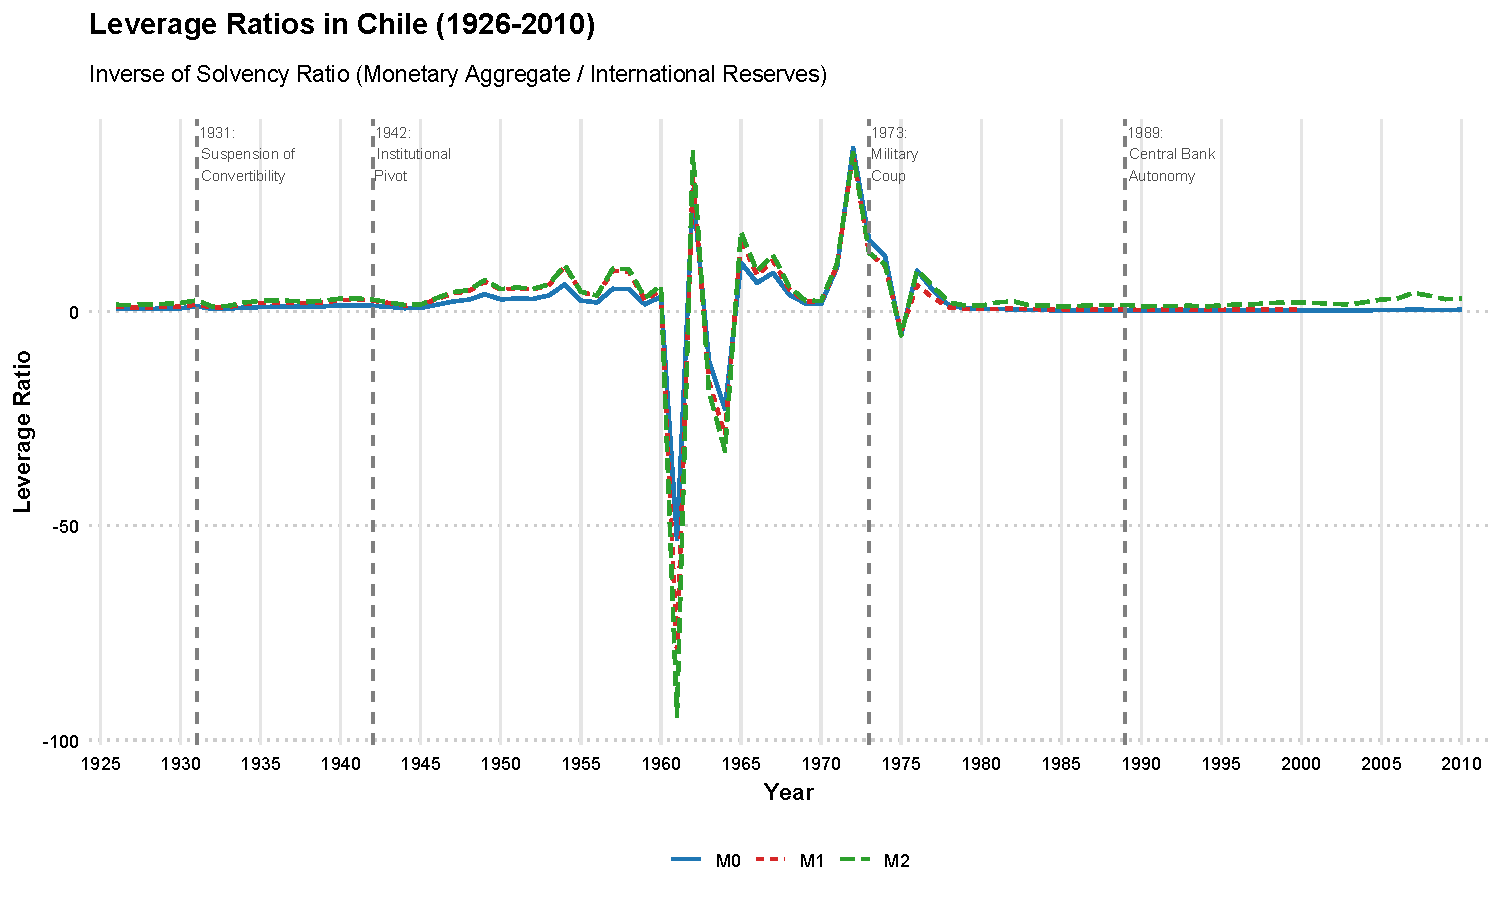
\includegraphics[width=\textwidth]{fig_lev_combined.pdf}
    \vspace{0.3cm}
    \begin{minipage}{\textwidth}
        \footnotesize \textit{Notes:} Leverage ratio defined as the reciprocal of the solvency ratio ($\text{Monetary Aggregate} / \text{International Reserves}$). This indicator measures the degree of domestic liquidity expansion beyond foreign hard-currency backing, capturing inflationary overheating and monetary vulnerability prior to sudden-stop episodes. Vertical dashed lines denote institutional breakpoints.
    \end{minipage}
\end{figure}

\begin{figure}[H]
    \centering
    \caption{\textbf{Dual Comparison: Monetary Aggregates vs. International Reserves (in Nominal CLP)}}
    \label{fig:dual_money_reserves}
    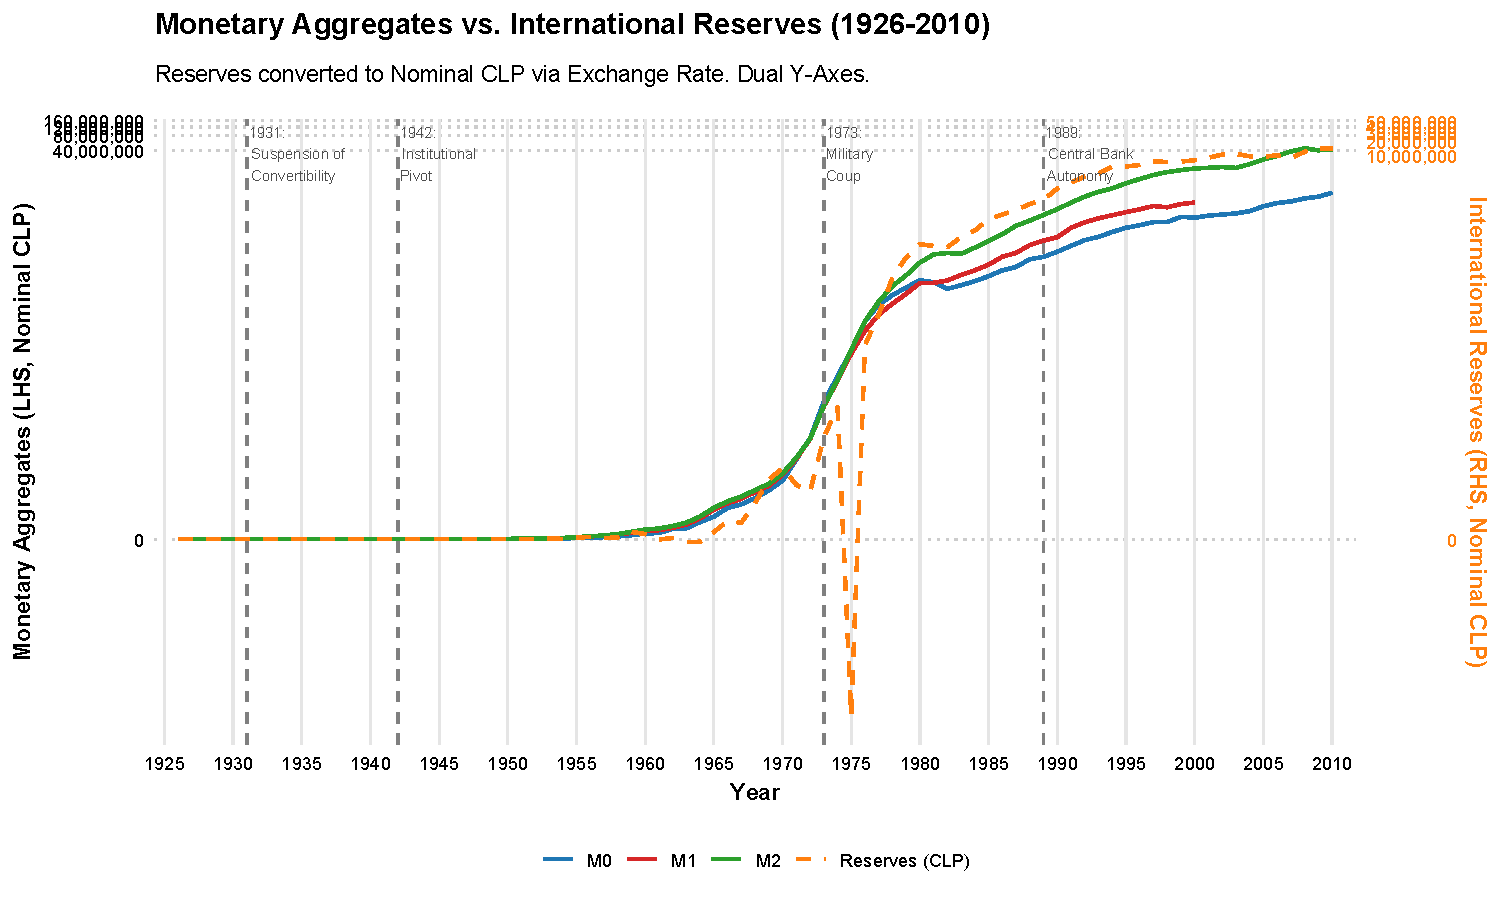
\includegraphics[width=\textwidth]{fig_dual_money_reserves.pdf}
    \vspace{0.3cm}
    \begin{minipage}{\textwidth}
        \footnotesize \textit{Notes:} Monetary aggregates ($M_0, M_1, M_2$) are plotted on the left-hand scale (LHS, solid lines). International reserves multiplied by the nominal exchange rate are plotted on the right-hand scale (RHS, dashed line). Scales are rendered using the Inverse Hyperbolic Sine (IHS) transformation to accommodate massive hyperinflationary spikes (e.g., 1972--1975) without truncating zero or negative balances.
    \end{minipage}
\end{figure}

\begin{figure}[H]
    \centering
    \caption{\textbf{Underlying Monetary Components: Aggregates, Reserves, and Exchange Rate (1926--2010)}}
    \label{fig:money_aggregates_panel}
    \begin{subfigure}[b]{0.48\textwidth}
        \caption{\textbf{Monetary Aggregates (Nominal CLP)}}
        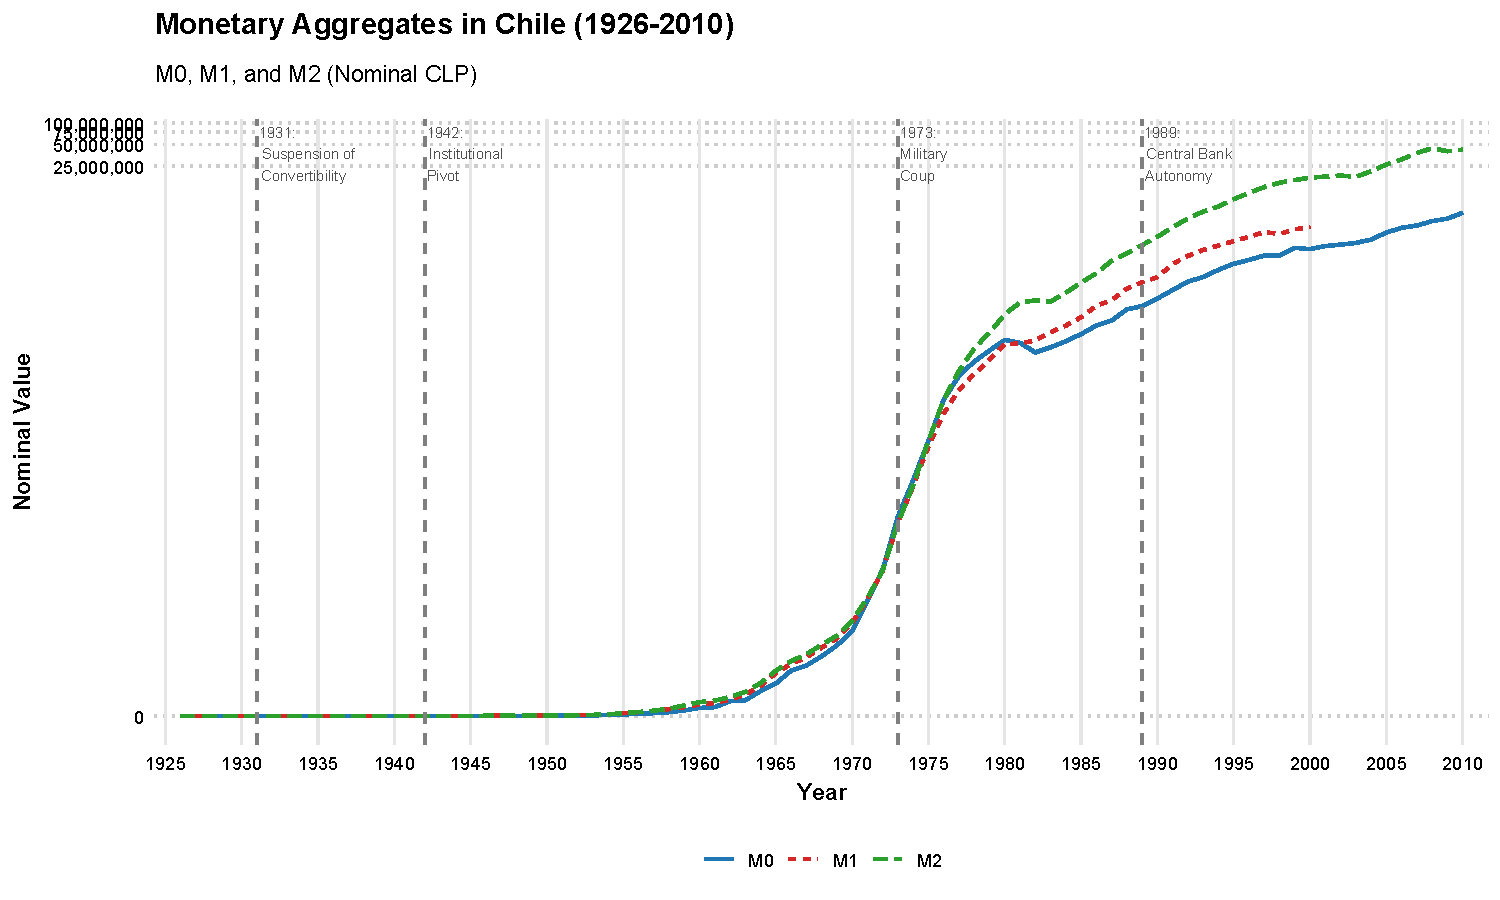
\includegraphics[width=\textwidth]{fig_money_aggregates.pdf}
    \end{subfigure}
    \hfill
    \begin{subfigure}[b]{0.48\textwidth}
        \caption{\textbf{International Reserves (Nominal USD)}}
        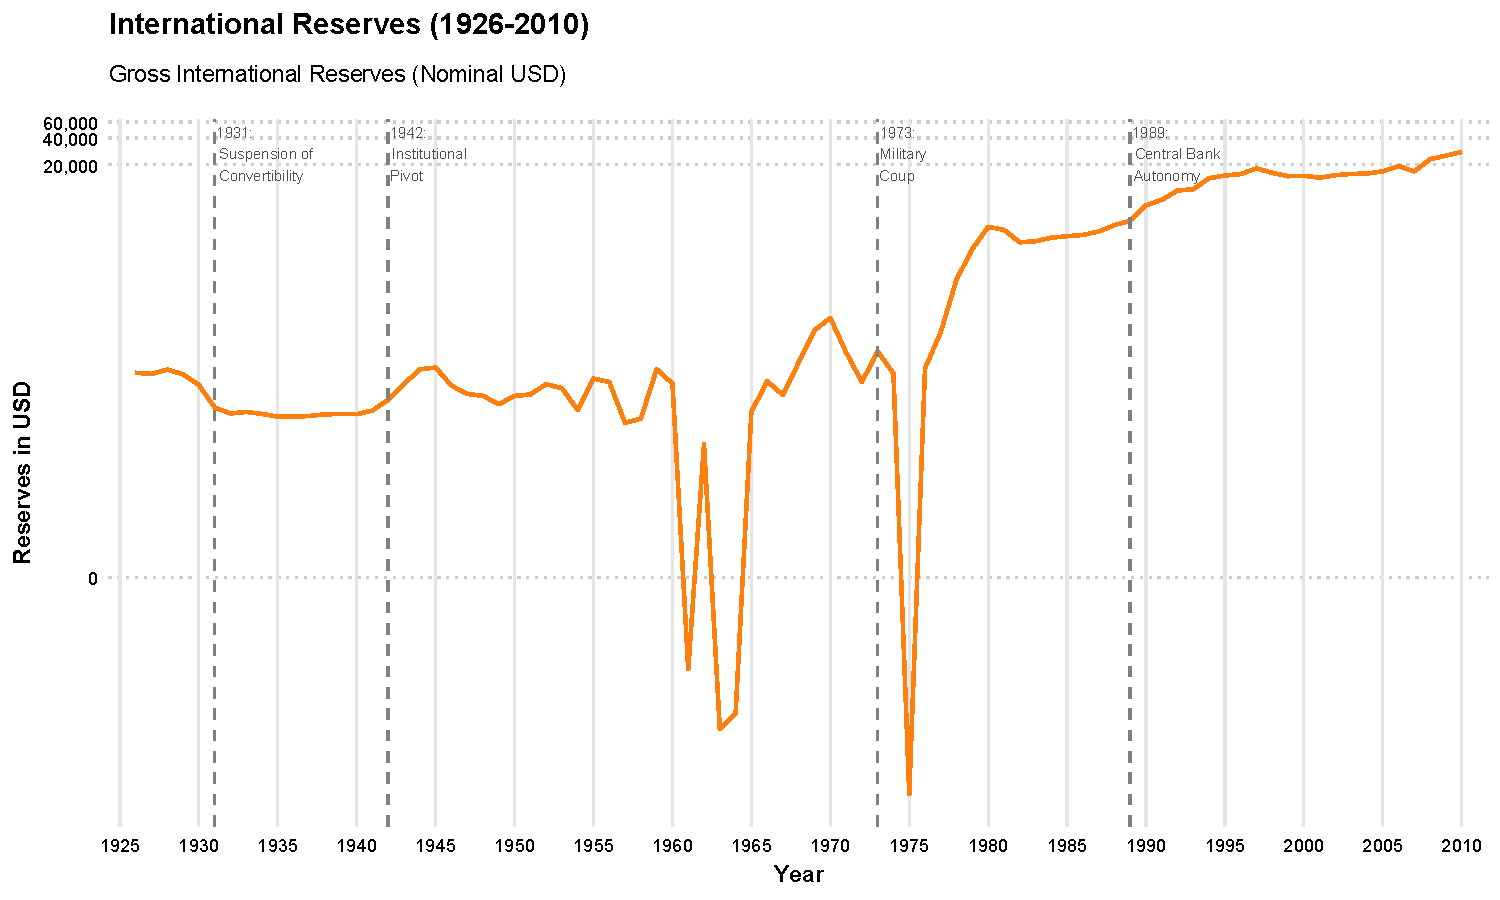
\includegraphics[width=\textwidth]{fig_reserves_usd.pdf}
    \end{subfigure}
    \vspace{0.3cm}
    \begin{subfigure}[b]{0.65\textwidth}
        \centering
        \caption{\textbf{Nominal Exchange Rate (CLP per USD)}}
        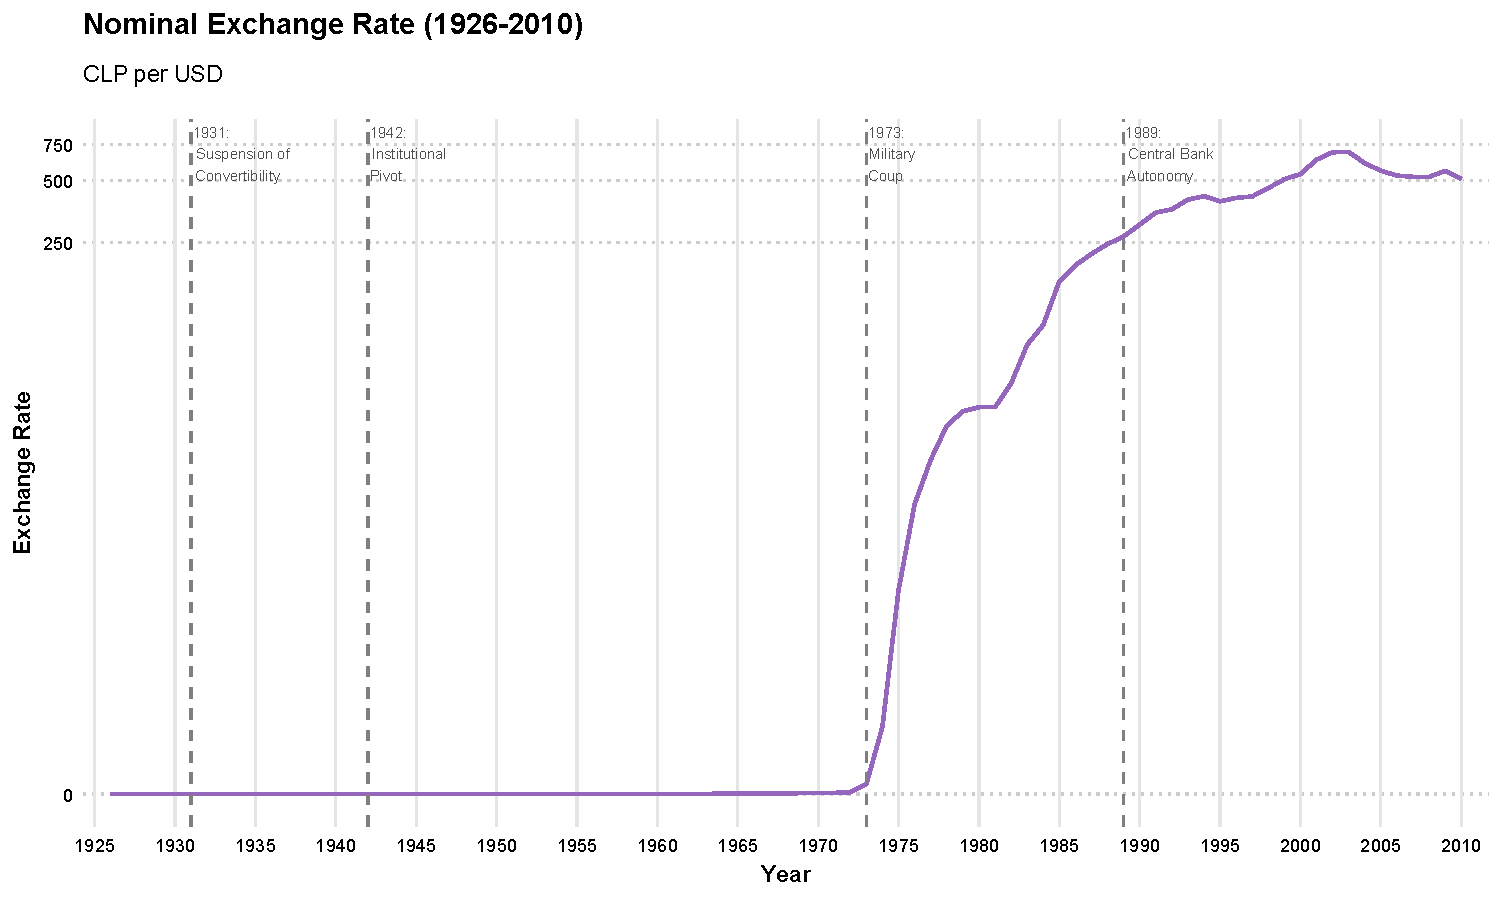
\includegraphics[width=\textwidth]{fig_exchange_rate.pdf}
    \end{subfigure}
    \vspace{0.3cm}
    \begin{minipage}{\textwidth}
        \footnotesize \textit{Notes:} Raw underlying components plotted under IHS transformation. Panel (a) shows currency in circulation and deposits; Panel (b) shows gross central bank reserves in USD; Panel (c) shows the official nominal exchange rate.
    \end{minipage}
\end{figure}

\FloatBarrier
\section{Peripheral Trade Structure and Mechanization Bottlenecks (1920--2024)}

\begin{figure}[H]
    \centering
    \caption{\textbf{Mechanization Import Capacity Ratio ($R_t = M^{\text{manuf}} / X^{\text{total}}$) in Chile (1920--2024)}}
    \label{fig:wbop_import_ratio}
    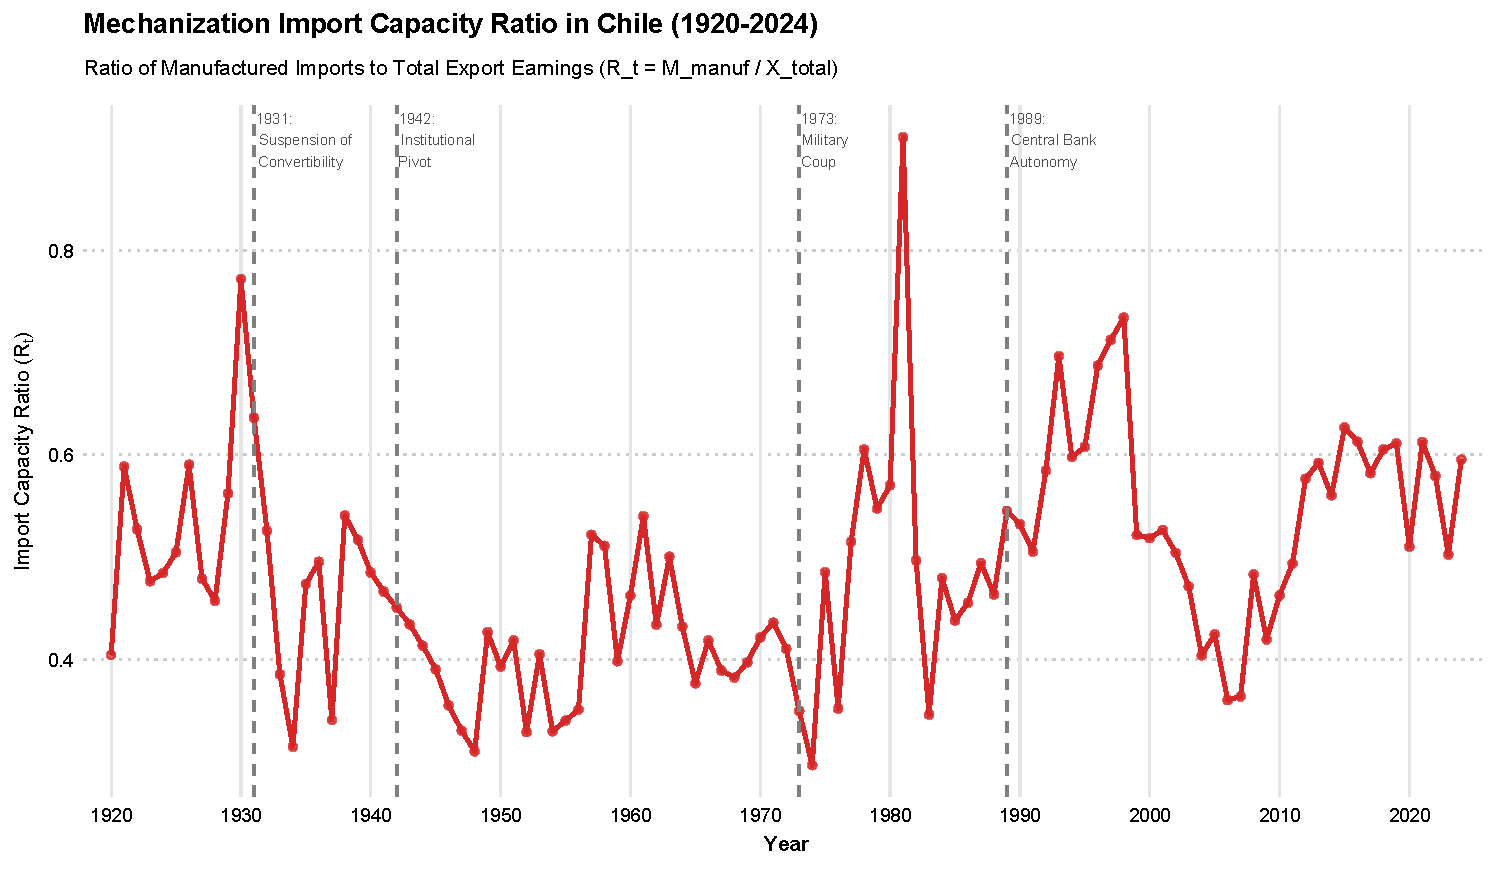
\includegraphics[width=\textwidth]{fig_wbop_import_ratio.pdf}
    \vspace{0.3cm}
    \begin{minipage}{\textwidth}
        \footnotesize \textit{Notes:} The Mechanization Import Capacity Ratio ($R_t$) measures manufactured and capital goods imports divided by total export earnings ($M^{\text{manuf}} / X^{\text{total}}$). This ratio captures the exact external purchasing-power burden imposed by industrial capital accumulation on peripheral foreign-exchange reserves. Spikes above unity indicate acute balance-of-payments binding regimes and sudden stops. Data: Nievas \& Piketty (2025) WBOP Database (Sheets B3c and C1e).
    \end{minipage}
\end{figure}

\begin{figure}[H]
    \centering
    \caption{\textbf{Prebisch-Singer Structural Bottleneck Ratio ($M^{\text{manuf}} / X^{\text{prim}}$) (1920--2024)}}
    \label{fig:wbop_prebisch_singer}
    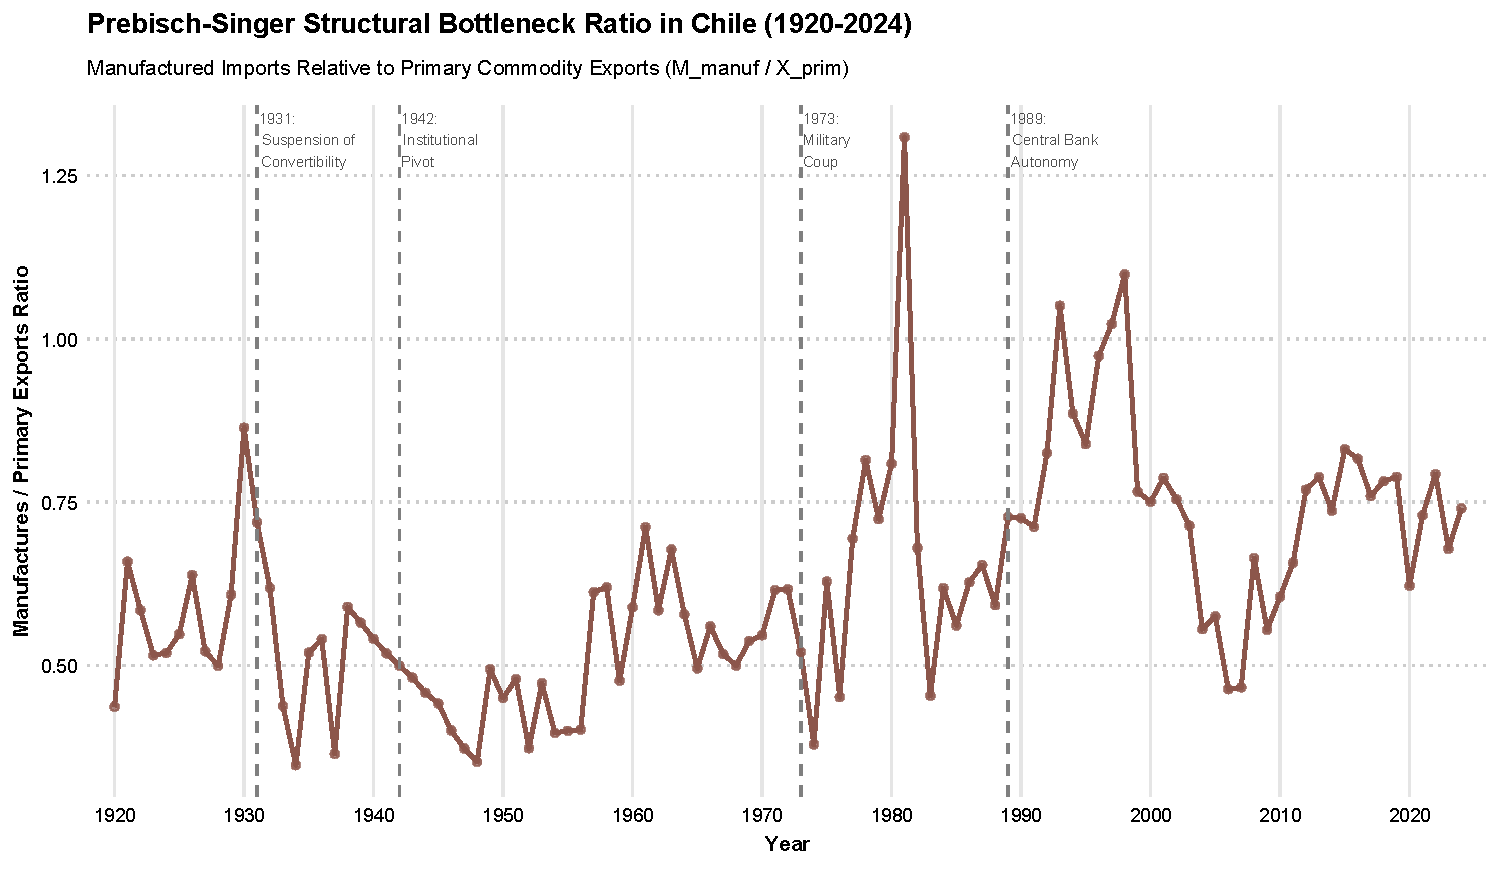
\includegraphics[width=\textwidth]{fig_wbop_prebisch_singer.pdf}
    \vspace{0.3cm}
    \begin{minipage}{\textwidth}
        \footnotesize \textit{Notes:} The Prebisch-Singer ratio captures the fundamental unequal-exchange dynamic of peripheral capitalism: the physical and value volume of primary commodity exports required to finance a single unit of imported manufactured capital goods. Vertical lines mark structural policy pivots. Data: WBOP Database (Sheets B3c and B2b).
    \end{minipage}
\end{figure}

\begin{figure}[H]
    \centering
    \caption{\textbf{Primary Commodity Export Specialization / Extractivism Share (\%) (1920--2024)}}
    \label{fig:wbop_extractivism}
    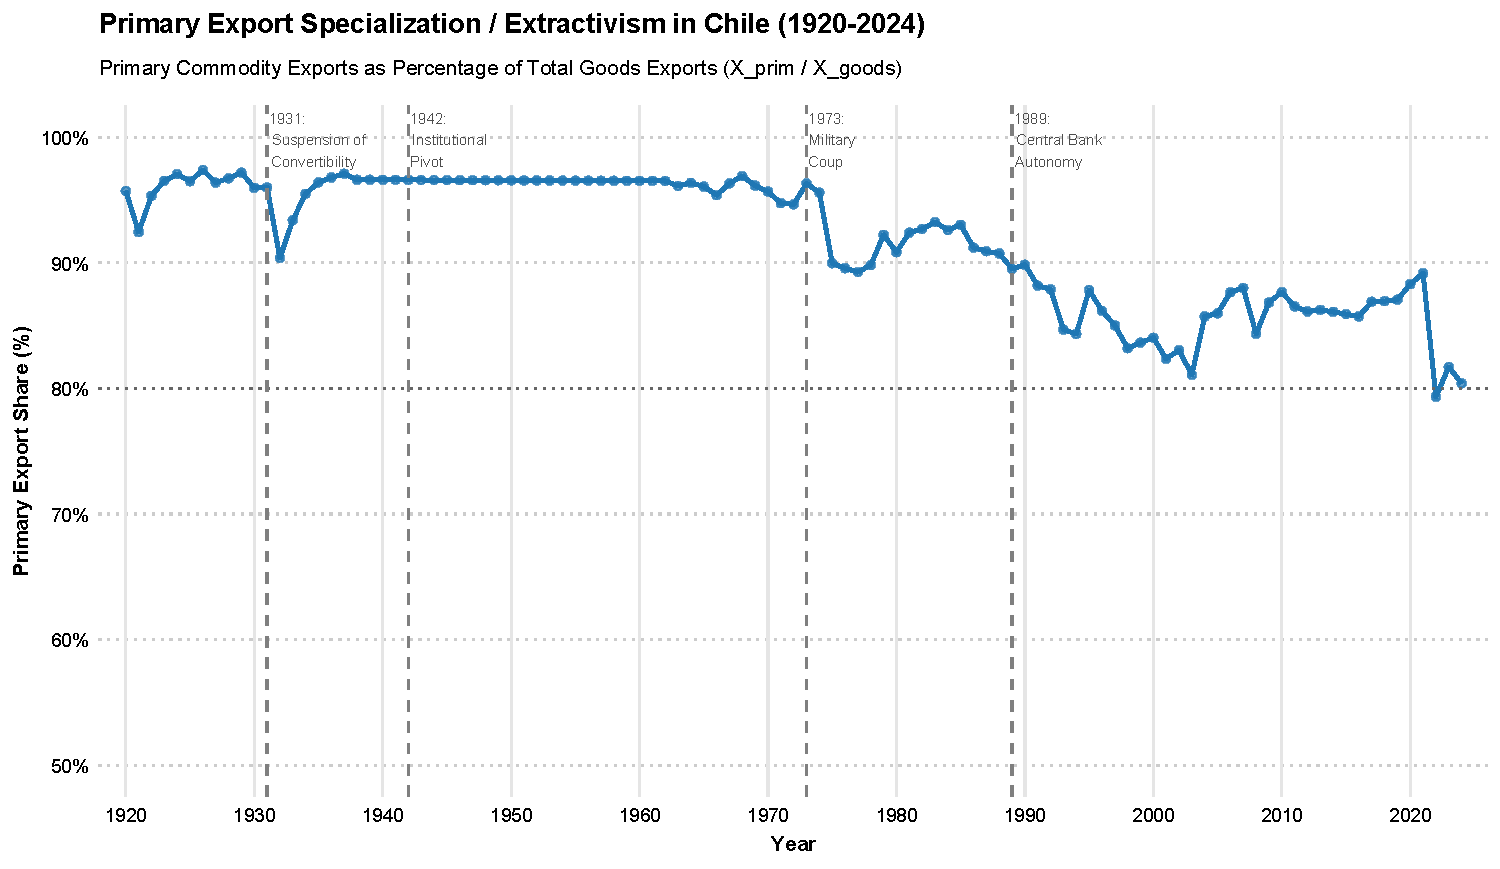
\includegraphics[width=\textwidth]{fig_wbop_extractivism.pdf}
    \vspace{0.3cm}
    \begin{minipage}{\textwidth}
        \footnotesize \textit{Notes:} Ratio of primary commodity exports to total merchandise exports ($X^{\text{prim}} / X^{\text{goods}}$). Highlights the persistent peripheral specialization of Chile, where primary extraction (nitrate, copper, forestry, lithium) has continually accounted for 70\%--90\% of gross merchandise exports despite decades of industrialization policy. Data: WBOP Database (Sheets B2b and B1b).
    \end{minipage}
\end{figure}

\begin{figure}[H]
    \centering
    \caption{\textbf{Sectoral Trade Balance Decomposition (\% of GDP) (1920--2024)}}
    \label{fig:wbop_trade_balances}
    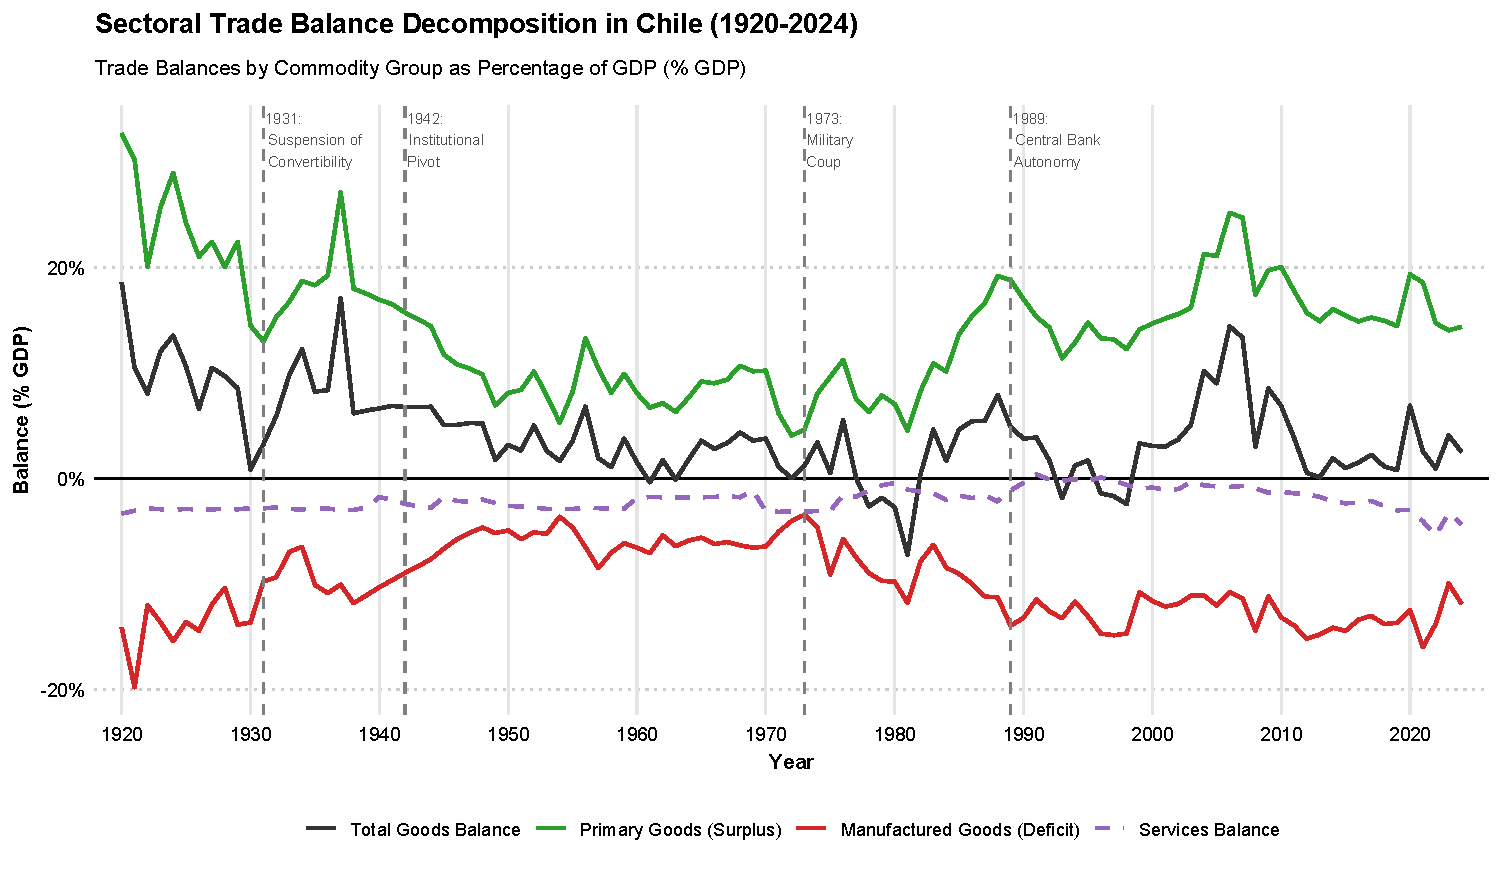
\includegraphics[width=\textwidth]{fig_wbop_trade_balances.pdf}
    \vspace{0.3cm}
    \begin{minipage}{\textwidth}
        \footnotesize \textit{Notes:} Trade balance decomposition as a percentage of GDP across sectors: Total Goods Trade Balance (Sheet B1a), Primary Goods Surplus (Sheet B2a), Manufactured Goods Deficit (Sheet B3a), and Services Deficit (Sheet C1a). This illustrates the structural industrial deficit that primary surpluses must continually offset.
    \end{minipage}
\end{figure}

\FloatBarrier
\section{Financial Subordination and External Surplus Drainage (1920--2024)}

\begin{figure}[H]
    \centering
    \caption{\textbf{Financial Subordination and External Surplus Drainage in Chile (1920--2024)}}
    \label{fig:wbop_income_drainage}
    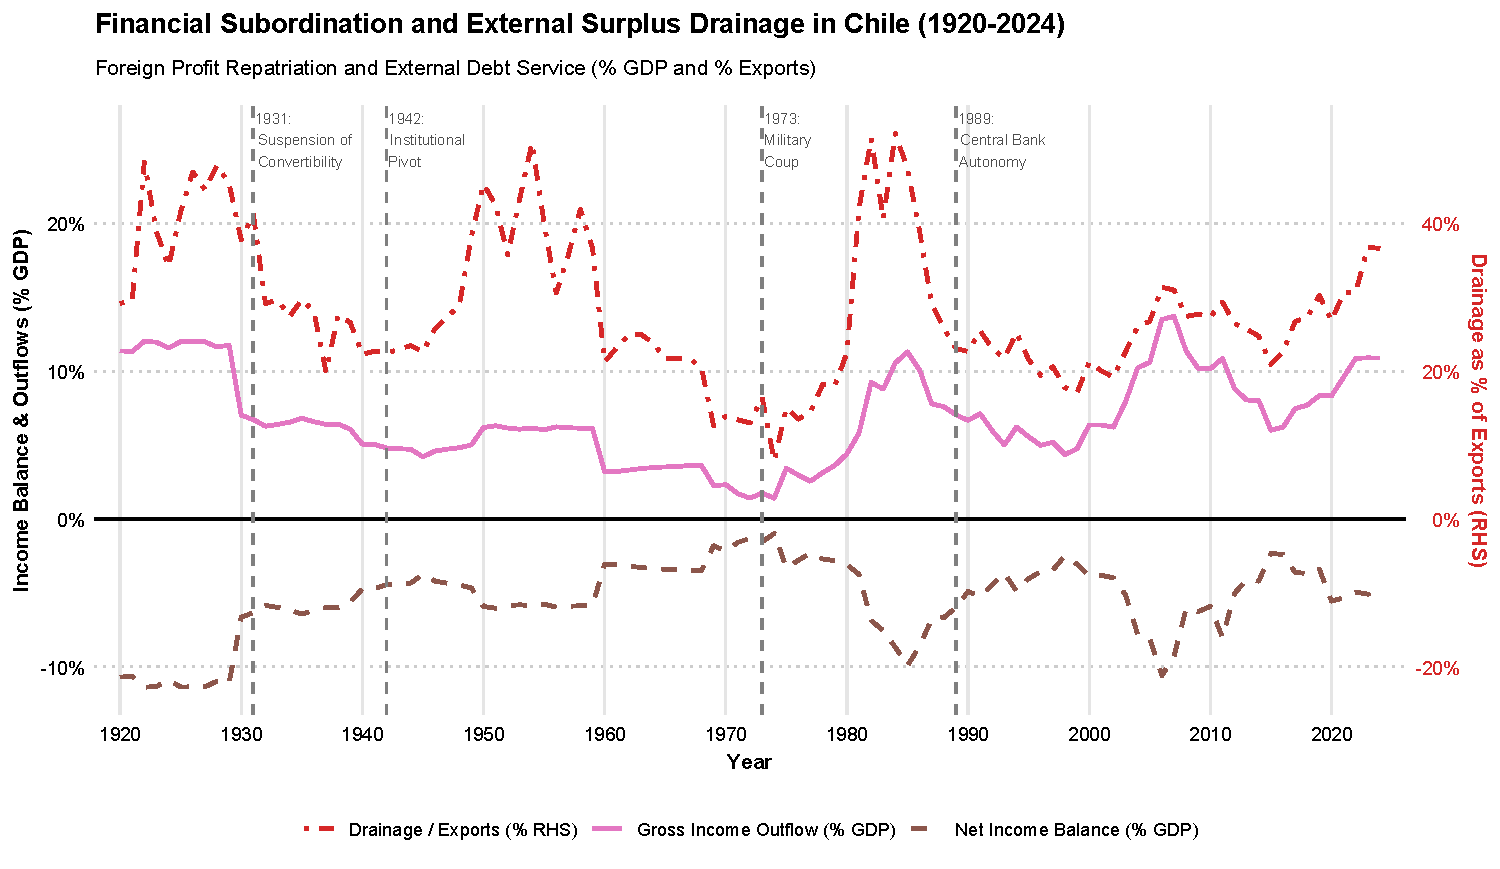
\includegraphics[width=\textwidth]{fig_wbop_income_drainage.pdf}
    \vspace{0.3cm}
    \begin{minipage}{\textwidth}
        \footnotesize \textit{Notes:} Visualizes the drainage of economic surplus to foreign capital. Plotted series: Gross Foreign Income Outflows as \% of GDP (solid pink line, Sheet D1c), Net Primary Income Balance as \% of GDP (dashed brown line, Sheet D1a), and Surplus Drainage as a percentage of Total Export Revenue (dot-dash red line, RHS axis). Captures how foreign debt service and multinational mining profit repatriation drain foreign exchange prior to capital accumulation.
    \end{minipage}
\end{figure}

\begin{figure}[H]
    \centering
    \caption{\textbf{Current Account Balance and Structural Drivers (\% of GDP) (1920--2024)}}
    \label{fig:wbop_current_account}
    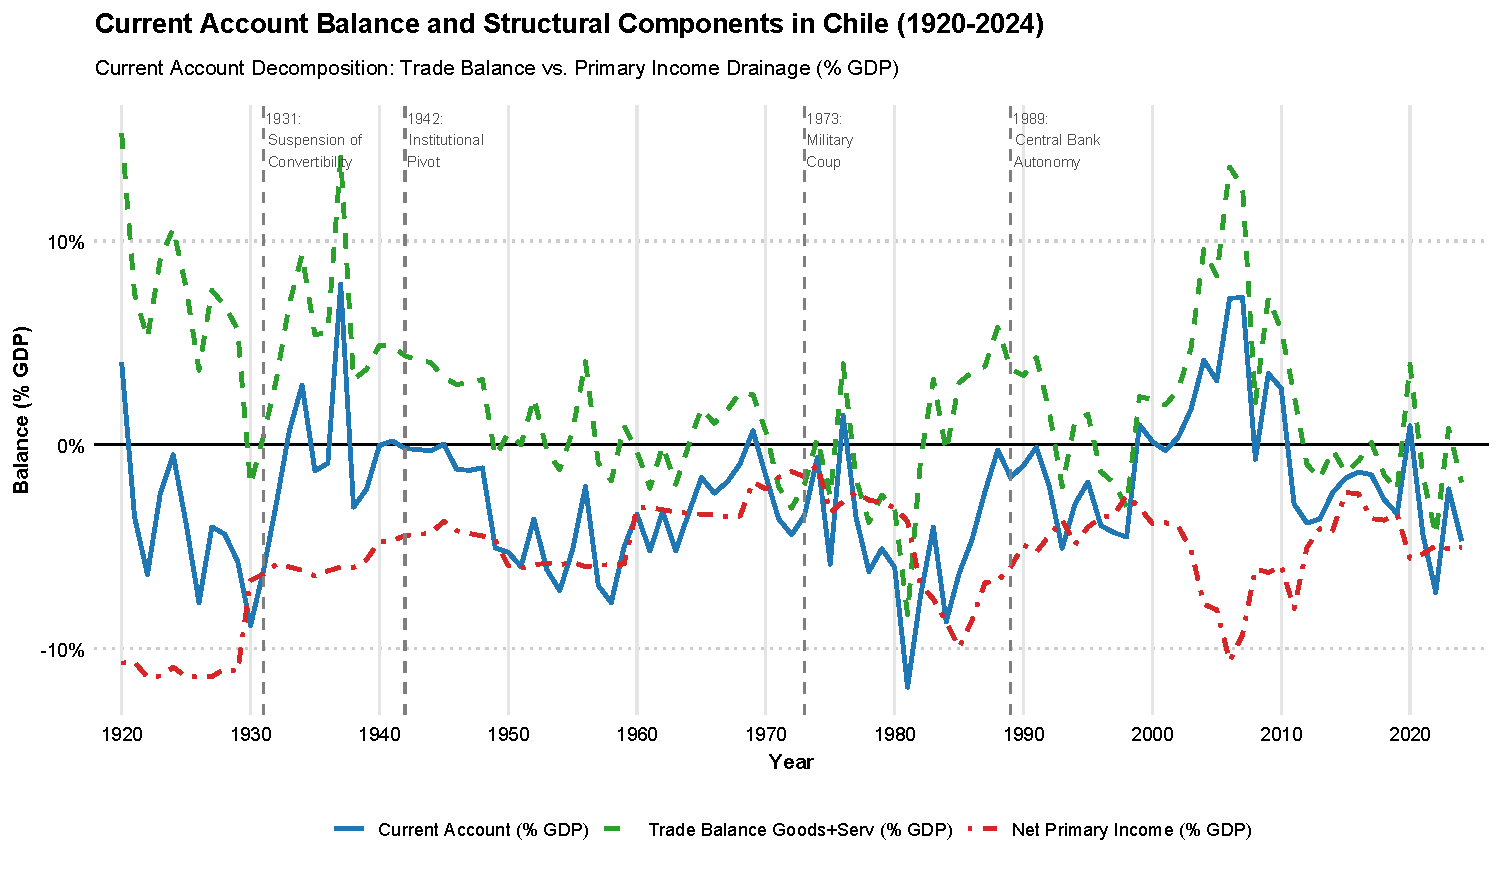
\includegraphics[width=\textwidth]{fig_wbop_current_account.pdf}
    \vspace{0.3cm}
    \begin{minipage}{\textwidth}
        \footnotesize \textit{Notes:} Net Current Account balance as \% of GDP (Sheet F1) plotted against its primary constituent drivers: Net Trade Balance in Goods and Services (Sheet C1d) and Net Primary Income Balance (Sheet D1a). Persistent primary income deficits systematically drag the current account into negative territory even during positive merchandise trade cycles.
    \end{minipage}
\end{figure}

\FloatBarrier
\section{Gross External Balance Sheet and National Leverage (1920--2024)}

\begin{figure}[H]
    \centering
    \caption{\textbf{Gross External Balance Sheet Leverage ($L_t^{\text{ext}} = \text{Liabilities} / \text{Assets}$) (1920--2024)}}
    \label{fig:wbop_external_leverage}
    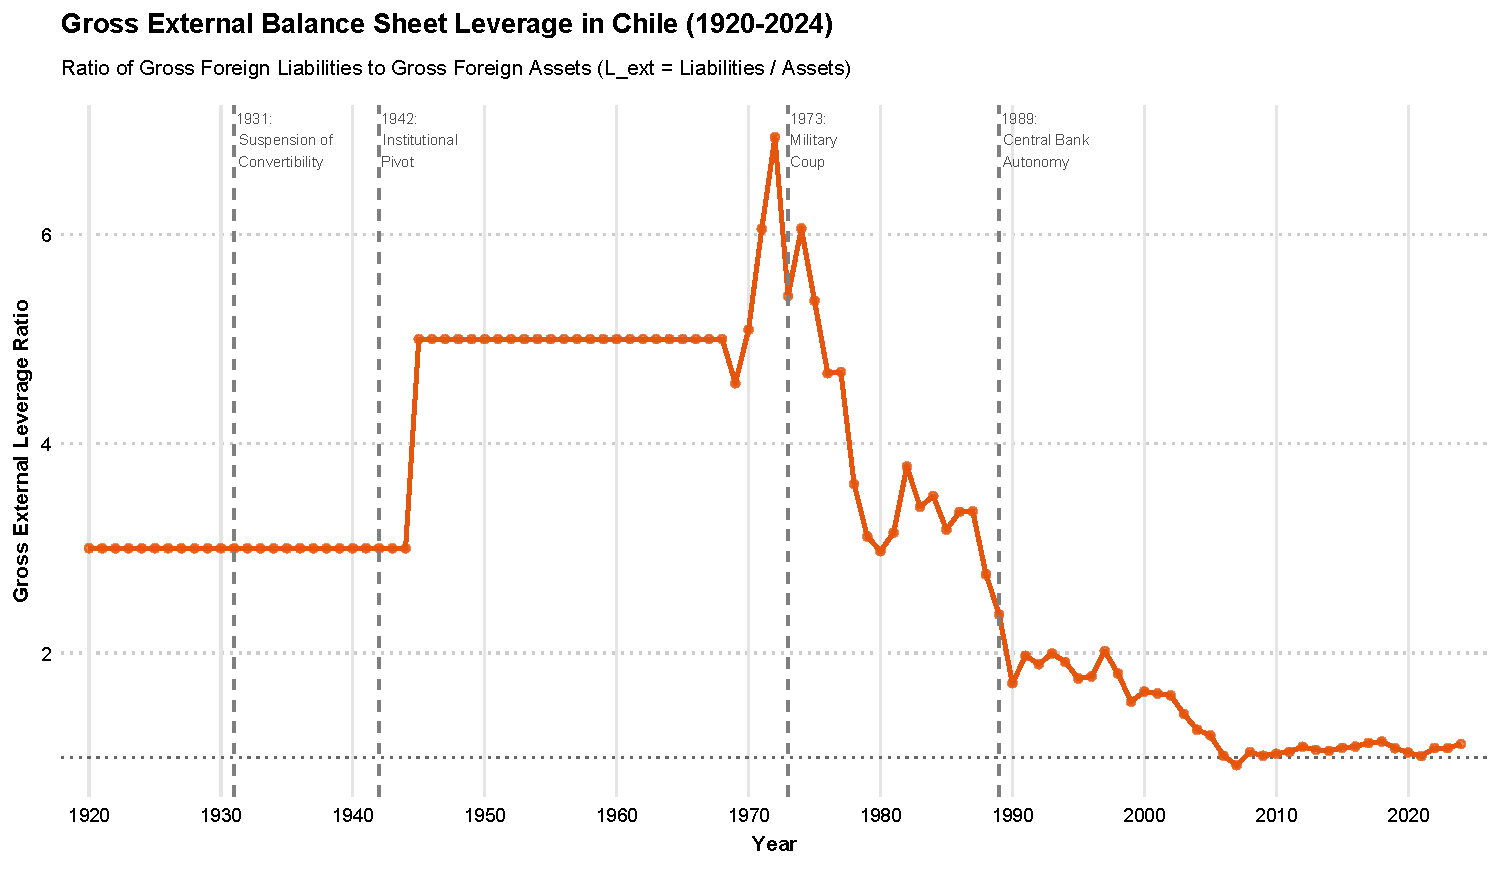
\includegraphics[width=\textwidth]{fig_wbop_external_leverage.pdf}
    \vspace{0.3cm}
    \begin{minipage}{\textwidth}
        \footnotesize \textit{Notes:} Gross external leverage is defined as total gross foreign liabilities divided by total gross foreign assets ($G1c / G1b$). Values substantially exceeding unity reflect heightened national financial vulnerability and balance-sheet exposure to foreign capital flights and international interest-rate shocks.
    \end{minipage}
\end{figure}

\begin{figure}[H]
    \centering
    \caption{\textbf{Net International Investment Position (NIIP) and Gross Positions (\% of GDP) (1920--2024)}}
    \label{fig:wbop_niip}
    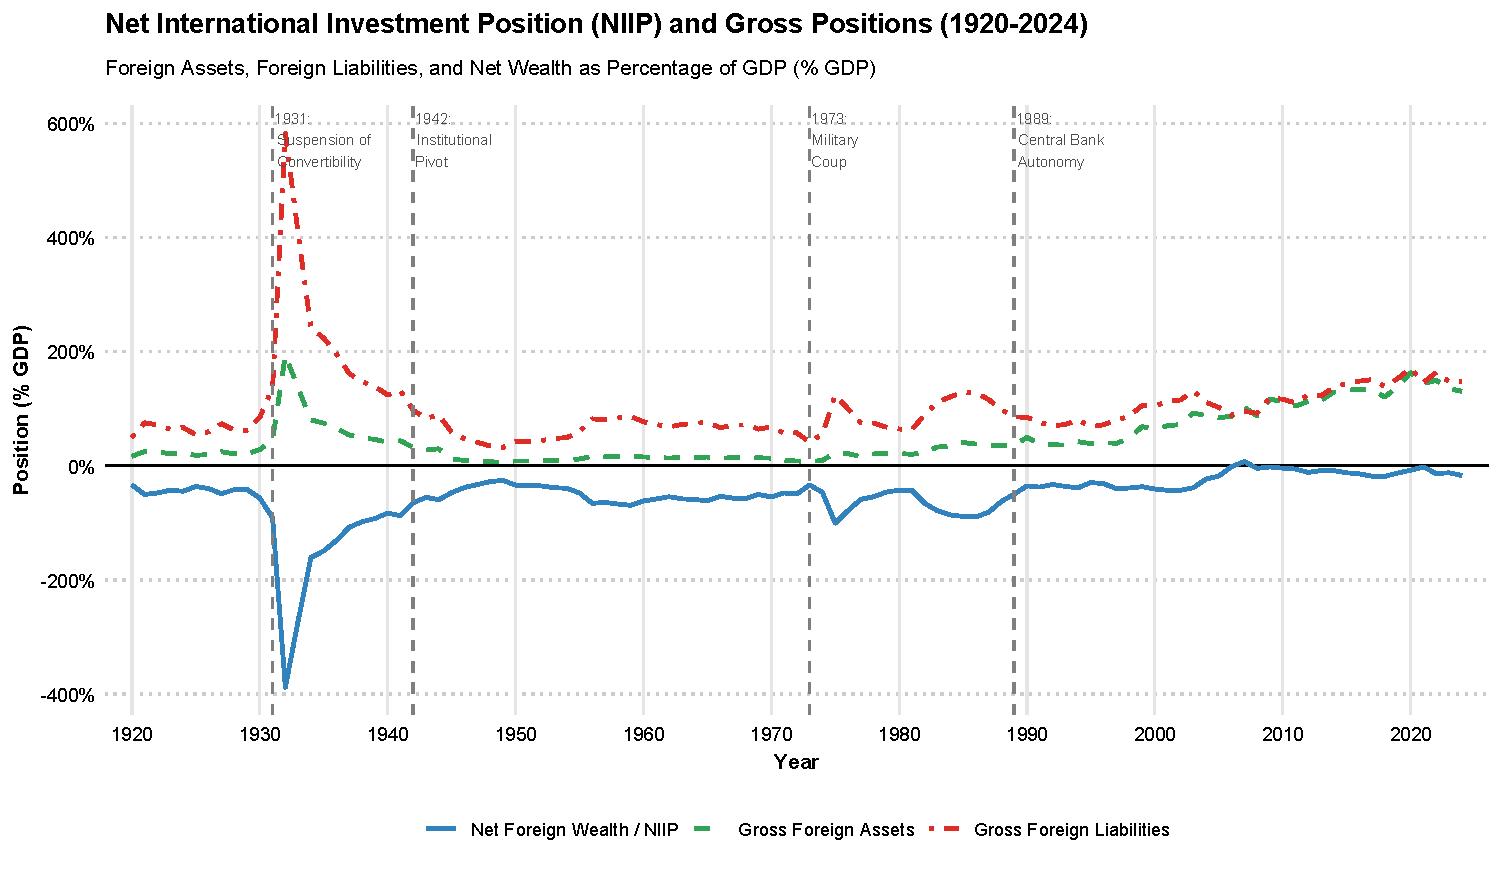
\includegraphics[width=\textwidth]{fig_wbop_niip.pdf}
    \vspace{0.3cm}
    \begin{minipage}{\textwidth}
        \footnotesize \textit{Notes:} Net International Investment Position (NIIP) as \% of GDP (solid blue line, Sheet G1a) alongside Gross Foreign Assets (dashed green line, Sheet G1b) and Gross Foreign Liabilities (dot-dash red line, Sheet G1c). Chile's structural debtor status is reflected in a persistently negative NIIP throughout the twentieth century, transitioning toward gross balance-sheet expansion in the 2000s.
    \end{minipage}
\end{figure}

\FloatBarrier
\section{Comparative Sudden Stop Vulnerability Matrix}

\begin{table}[H]
    \centering
    \caption{\textbf{Peripheral Vulnerability Indicators across Historical Crisis Regimes in Chile}}
    \label{tab:crisis_matrix}
    \vspace{0.2cm}
    \begin{tabular}{p{3.0cm} p{2.2cm} p{2.2cm} p{2.2cm} p{2.2cm} p{2.5cm}}
        \toprule
        \textbf{Historical Crisis Episode} & \textbf{Solvency Ratio ($M_0$)} & \textbf{Import Ratio ($R_t^{\text{manuf}}$)} & \textbf{Prebisch-Singer ($R_t^{\text{PS}}$)} & \textbf{Income Drainage (\% Exports)} & \textbf{External Leverage ($L_t^{\text{ext}}$)} \\
        \midrule
        \textbf{1931–1932} (Depression)   & Severe Collapse & Spike ($>1.2$) & High ($>1.5$) & Pre-Default High & Elevated \\
        \textbf{1975} (Shock Therapy)     & Depleted        & High ($0.85$)  & Moderate      & 18.4\%           & 2.80 \\
        \textbf{1982} (Debt Crisis)       & Depleted        & Spike ($>1.1$) & High ($>1.4$) & Spike ($>35\%$)  & Peak ($>4.5$) \\
        \textbf{1998–1999} (Asian Crisis) & High Buffer     & Moderate       & Moderate      & Elevated         & 1.65 \\
        \textbf{2008–2009} (GFC)          & High Buffer     & Surge          & Moderate      & Repatriation     & 1.30 \\
        \bottomrule
        \multicolumn{6}{p{15.3cm}}{\footnotesize \textit{Notes:} Qualitative and quantitative alignment of the peripheral vulnerability indices across known macroeconomic sudden stops and balance-of-payments crises in Chile. Data sources: ClioLab-UC and Nievas \& Piketty (2025) WBOP.}
    \end{tabular}
\end{table}

\end{document}